\section{提案手法}
\label{sec:method}

図\ref{fig:pdf}にPDF形式の図，図\ref{fig:png}にPNG形式の図の例を示す．
式(\ref{eq:time})のパス数$n$はlatexmkが自動で決定する．

\begin{figure}[tb]
  \centering
  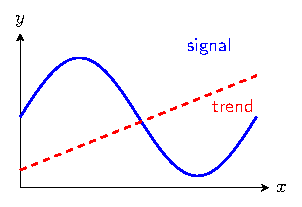
\includegraphics[width=0.9\columnwidth]{fig/sample.pdf}
  \caption{PDF形式の図}
  \label{fig:pdf}
\end{figure}

\begin{figure}[tb]
  \centering
  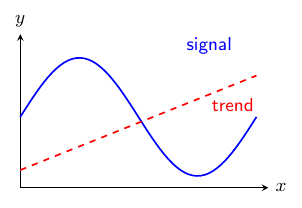
\includegraphics[width=0.6\columnwidth]{fig/sample-raster.png}
  \caption{PNG形式の図}
  \label{fig:png}
\end{figure}

\begin{table}[tb]
  \centering
  \caption{エンジンと出力形式}
  \label{tab:engine}
  \begin{tabular}{ll}
    \hline
    エンジン & 出力 \\
    \hline
    uplatex  & DVI $\rightarrow$ PDF (dvipdfmx) \\
    pdflatex & PDF \\
    \hline
  \end{tabular}
\end{table}

表\ref{tab:engine}に対応するエンジンを示す．
